% Options for packages loaded elsewhere
\PassOptionsToPackage{unicode}{hyperref}
\PassOptionsToPackage{hyphens}{url}
%
\documentclass[
]{article}
\usepackage{amsmath,amssymb}
\usepackage{iftex}
\ifPDFTeX
  \usepackage[T1]{fontenc}
  \usepackage[utf8]{inputenc}
  \usepackage{textcomp} % provide euro and other symbols
\else % if luatex or xetex
  \usepackage{unicode-math} % this also loads fontspec
  \defaultfontfeatures{Scale=MatchLowercase}
  \defaultfontfeatures[\rmfamily]{Ligatures=TeX,Scale=1}
\fi
\usepackage{lmodern}
\ifPDFTeX\else
  % xetex/luatex font selection
\fi
% Use upquote if available, for straight quotes in verbatim environments
\IfFileExists{upquote.sty}{\usepackage{upquote}}{}
\IfFileExists{microtype.sty}{% use microtype if available
  \usepackage[]{microtype}
  \UseMicrotypeSet[protrusion]{basicmath} % disable protrusion for tt fonts
}{}
\makeatletter
\@ifundefined{KOMAClassName}{% if non-KOMA class
  \IfFileExists{parskip.sty}{%
    \usepackage{parskip}
  }{% else
    \setlength{\parindent}{0pt}
    \setlength{\parskip}{6pt plus 2pt minus 1pt}}
}{% if KOMA class
  \KOMAoptions{parskip=half}}
\makeatother
\usepackage{xcolor}
\usepackage[margin=1in]{geometry}
\usepackage{longtable,booktabs,array}
\usepackage{calc} % for calculating minipage widths
% Correct order of tables after \paragraph or \subparagraph
\usepackage{etoolbox}
\makeatletter
\patchcmd\longtable{\par}{\if@noskipsec\mbox{}\fi\par}{}{}
\makeatother
% Allow footnotes in longtable head/foot
\IfFileExists{footnotehyper.sty}{\usepackage{footnotehyper}}{\usepackage{footnote}}
\makesavenoteenv{longtable}
\usepackage{graphicx}
\makeatletter
\def\maxwidth{\ifdim\Gin@nat@width>\linewidth\linewidth\else\Gin@nat@width\fi}
\def\maxheight{\ifdim\Gin@nat@height>\textheight\textheight\else\Gin@nat@height\fi}
\makeatother
% Scale images if necessary, so that they will not overflow the page
% margins by default, and it is still possible to overwrite the defaults
% using explicit options in \includegraphics[width, height, ...]{}
\setkeys{Gin}{width=\maxwidth,height=\maxheight,keepaspectratio}
% Set default figure placement to htbp
\makeatletter
\def\fps@figure{htbp}
\makeatother
\setlength{\emergencystretch}{3em} % prevent overfull lines
\providecommand{\tightlist}{%
  \setlength{\itemsep}{0pt}\setlength{\parskip}{0pt}}
\setcounter{secnumdepth}{-\maxdimen} % remove section numbering
\ifLuaTeX
  \usepackage{selnolig}  % disable illegal ligatures
\fi
\usepackage{bookmark}
\IfFileExists{xurl.sty}{\usepackage{xurl}}{} % add URL line breaks if available
\urlstyle{same}
\hypersetup{
  pdftitle={Stomach vs.~Liver Transcriptomic Analysis},
  hidelinks,
  pdfcreator={LaTeX via pandoc}}

\title{Stomach vs.~Liver Transcriptomic Analysis}
\usepackage{etoolbox}
\makeatletter
\providecommand{\subtitle}[1]{% add subtitle to \maketitle
  \apptocmd{\@title}{\par {\large #1 \par}}{}{}
}
\makeatother
\subtitle{BINF694 - Interim Report}
\author{}
\date{\vspace{-2.5em}April 22, 2025}

\begin{document}
\maketitle

\section{Introduction}\label{introduction}

The human body is comprised of diverse organs with specialized functions
that are ultimately reflected in their gene expression profiles. Of
these, the liver and stomach represent two distinct but complementary
filtering systems that process what enters the body. Transcriptomic
analysis allows us to see these underling specialized functions at the
genomic level.

The liver serves as the body's primary detoxification center, filtering
blood. It synthesizes essential proteins including albumin and clotting
factors, and maintains glucose homeostasis through glycogen storage and
gluconeogenesis (Rui, 2014). These functions require coordinated
expression of genes encoding cytochrome P450 enzymes, transporters like
ABCC2, and serum proteins such as alpha-1 antitrypsin (AAT).

In contrast, the stomach functions as the initial filtering station for
ingested materials. Its specialized epithelium includes parietal cells
that secrete hydrochloric acid (HCl) via H+/K+-ATPase pumps (ATP4A,
ATP4B), chief cells producing pepsinogen, and mucus-secreting cells that
protect the stomach lining (Mills \& Shivdasani, 2011). This acidic
environment serves as both a chemical barrier against pathogens and
initiates protein digestion.

This hypothesizes that the liver and stomach will show differentially
expressed gene patterns reflecting their specialized filtering
functions, with the liver expressing higher levels of detoxification and
metabolic pathway genes, while the stomach will show elevated expression
of genes related to acid production, mucus secretion, and initial
digestive processes. Through RNA-sequencing analysis of three biological
replicates from each tissue, we aim to characterize these distinct
transcriptomic signatures and identify the key molecular pathways that
distinguish these filtering organs.

\subsection{Hypothesis}\label{hypothesis}

The liver and stomach will show differentially expressed gene patterns
reflecting their specialized filtering functions. The liver will express
higher levels of detoxification and metabolic pathway genes; while the
stomach will show elevated expression of genes related to acid
production, mucus secretion, and initial digestive processes.

\section{Methods}\label{methods}

Three biological replicates each of human liver (samples a, c, and d)
and stomach (samples 1a, 2a, and 3b) tissues were selected for
comparative transcriptomic analysis. The analysis aimed to test the
hypothesis that liver and stomach tissues would show differentially
expressed gene patterns reflecting their specialized filtering
functions, with the liver expressing higher levels of detoxification and
metabolic pathway genes, while the stomach would show elevated
expression of genes related to acid production, mucus secretion, and
initial digestive processes.

Claude 3.7
Sonnet{[}\url{https://claude.ai/share/5142901c-bf60-4d6b-a944-a95c549ac000}{]}

\subsection{Qualitiy Control}\label{qualitiy-control}

The first step was to perform quality control analysis on the 6 tissue
samples using FastQC. The selected samples were analyzed using version
0.11.9 of FastQC. Quality metrics including per base sequence quality,
per sequence quality scores, sequence duplication levels, adapter
content, and k-mer content were evaluated.

\paragraph{Liver Tissue Analysis}\label{liver-tissue-analysis}

Overall the three liver samples analyzed expressed similar results.
There were no concerns with the results from samples a and c, however,
with sample d there is some concern with a substantial proportion of
bases had quality scores below 28, which led to higher filtering rates
during trimming.

\paragraph{Stomach Tissue Analysis}\label{stomach-tissue-analysis}

Similar to the liver tissues, two stomach samples (1a and 2a) showed
satisfactory quality metrics. Sample 3b exhibited quality concerns with
a larger proportion of bases below quality score 28, resulting in more
aggressive filtering during trimming.

\subsection{Trimming}\label{trimming}

\begin{longtable}[]{@{}ll@{}}
\caption{Trimming Results \textbar{} Table 1}\tabularnewline
\toprule\noalign{}
sample & Remaining.Percentage \\
\midrule\noalign{}
\endfirsthead
\toprule\noalign{}
sample & Remaining.Percentage \\
\midrule\noalign{}
\endhead
\bottomrule\noalign{}
\endlastfoot
liver\_a & 90.50\% \\
liver\_c & 91.40\% \\
liver\_d & 79.70\% \\
stomach\_a & 90.70\% \\
stomach\_3a & 87.90\% \\
stomach\_3b & 81.30\% \\
\end{longtable}

After it was determined that we can proceed with further analysis of the
provided samples, FastQC was utilized to trim the samples. The samples
were filtered on a minimum read length of 40 and a quality score of 28.
This will allow us to retain the sequences meeting our quality
threshold.

As expected, liver\_d and stomach\_3b had the highest proportion of
sequences filtered out during this step, consistent with their lower
initial quality metrics.

\subsection{Mapping}\label{mapping}

\begin{longtable}[]{@{}
  >{\raggedright\arraybackslash}p{(\columnwidth - 6\tabcolsep) * \real{0.1429}}
  >{\raggedright\arraybackslash}p{(\columnwidth - 6\tabcolsep) * \real{0.2727}}
  >{\raggedright\arraybackslash}p{(\columnwidth - 6\tabcolsep) * \real{0.1948}}
  >{\raggedright\arraybackslash}p{(\columnwidth - 6\tabcolsep) * \real{0.3896}}@{}}
\caption{Mapping Results \textbar{} Table 2}\tabularnewline
\toprule\noalign{}
\begin{minipage}[b]{\linewidth}\raggedright
sample
\end{minipage} & \begin{minipage}[b]{\linewidth}\raggedright
mapped\_reads\_percent
\end{minipage} & \begin{minipage}[b]{\linewidth}\raggedright
missmatch\_rate
\end{minipage} & \begin{minipage}[b]{\linewidth}\raggedright
mapped\_multi\_location\_percent
\end{minipage} \\
\midrule\noalign{}
\endfirsthead
\toprule\noalign{}
\begin{minipage}[b]{\linewidth}\raggedright
sample
\end{minipage} & \begin{minipage}[b]{\linewidth}\raggedright
mapped\_reads\_percent
\end{minipage} & \begin{minipage}[b]{\linewidth}\raggedright
missmatch\_rate
\end{minipage} & \begin{minipage}[b]{\linewidth}\raggedright
mapped\_multi\_location\_percent
\end{minipage} \\
\midrule\noalign{}
\endhead
\bottomrule\noalign{}
\endlastfoot
liver\_a & 92.37\% & 0.14\% & 6.90\% \\
liver\_c & 93.86\% & 0.13\% & 5.49\% \\
liver\_d & 93.14\% & 0.22\% & 6.22\% \\
stomach\_a & 90.05\% & 0.27\% & 6.99\% \\
stomach\_3a & 88.25\% & 0.29\% & 9.06\% \\
stomach\_3b & 77.52\% & 0.28\% & 21.08\% \\
\end{longtable}

Using the filtered sequences, STAR version 2.7.11b was utilized to align
the sequences in the genome. The results from the mapping were not
concerning. Overall, there was a higher mismatch rate for the stomach
tissue samples. The may also be some quality issues with stomach\_3b as
the mapping rate of about 77.5\% is pretty low. This may indicate some
contamination in the sample as well as the multi mapping rate was much
higher than the other tissue samples.

SAMtools version 1.19.2 was then used to create the .bam files that will
be used for counting.

\subsection{Genome Visulization}\label{genome-visulization}

Integrative Genomics Viewer (IGV) version 2.8.0 was used to visualize
read alignments for genes of interest, allowing for inspection of exon
coverage patterns and verification of expression differences between
liver and stomach tissues.

\subsection{Read Counting}\label{read-counting}

HTSeq version 0.11.2 was used to count the 6 sorted and aligned .bam
file provided by trimming and mapping.

\textbf{Paramaters:}

\begin{verbatim}
mode intersection-nonempty
stranded no
format bam
type exon
idattr gene_name
\end{verbatim}

\subsection{Differential Expression
Analysis}\label{differential-expression-analysis}

Differential expression analysis was performed using DESeq2 version
1.38.0 in R version 4.2.0. 1. Via a created count matrix from the six
tissue counts, a DESeqDataSet object was created 2. Low-count genes
(those with fewer than 10 reads across all samples) were filtered out 3.
Results were ordered by adjusted p-value and exported to a tab-delimited
file

\subsection{Understanding Sample
Relationships}\label{understanding-sample-relationships}

\begin{itemize}
\tightlist
\item
  Principal Component Analysis (PCA) on variance-stabilized transformed
  data (vst) from DESeq2
\item
  Sample distance matrix visualized as a heatmap with hierarchical
  clustering
\item
  Multi-Dimensional Scaling (MDS) plot from edgeR to assess sample
  relationships
\item
  Heatmaps of the top 50 differentially expressed genes across all
  samples
\item
  MA plots to show the relationship between mean expression and log2
  fold change
\item
  Smear plots from edgeR to visualize differentially expressed genes
\end{itemize}

Additionally, selected marker genes from various research publications
were analyzed separately and visualized in a heatmap with row-based
scaling to highlight expression patterns.

\subsection{Enrichment Analysis}\label{enrichment-analysis}

\textbf{DAVID (Database for Annotation, Visualization and Integrated
Discovery) version 6.8}

\begin{itemize}
\item
  Functional annotation
\item
  Ontology

  \begin{itemize}
  \tightlist
  \item
    Biological process
  \item
    molecular function
  \item
    cellular component
  \end{itemize}
\item
  KEGG pathways
\end{itemize}

\textbf{Enrichr}

\begin{itemize}
\tightlist
\item
  GO Biological
\item
  KEGG 2021 Human
\item
  WikiPathways 2023 Human
\end{itemize}

NOT DONE!

\newpage

\section{Results}\label{results}

\subsection{Sample Relationship}\label{sample-relationship}

The Principle component analysis (PCA) plot further confirms the
distinct transcriptomic profiles between liver and stomach samples in
your analysis. This PCA plot provides a dimensionality reduction
visualization of your RNA-seq data after variance stabilizing
transformation.

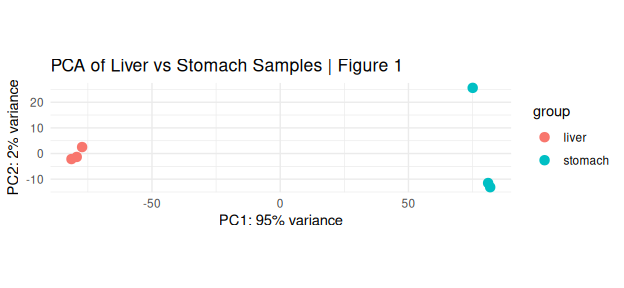
\includegraphics{InterimAnalysis_files/figure-latex/fig1_pca-1.pdf} The
extreme separation along PC1 (which captures 95\% of variance) provides
enough evidence that the profiles of liver and stomach are fundamentally
different, supporting your hypothesis about their distinct filtering
functions. This is consistent with the expected biological differences
between these organs, with liver specialized for blood
filtration/detoxification and stomach for food processing. The large
proportion of variance explained by PC1 suggests there are strongly
differentially expressed genes between these tissues, which should
provide rich material for pathway and functional analysis.

Next we will use a heatmap to visualize the clustering of samples by
tissue type.

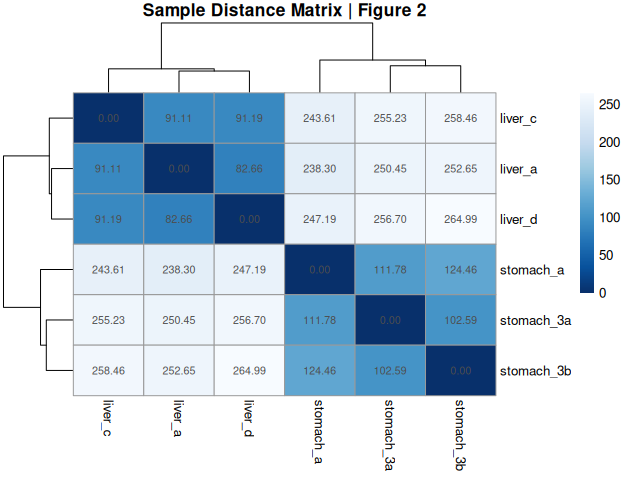
\includegraphics{InterimAnalysis_files/figure-latex/fig2_heatmap-1.pdf}
The heatmap shows a hierarchical clustering of your six samples based on
their gene expression profiles after variance stabilizing
transformation. The numerical values represent Euclidean distances
between samples, with darker blue indicating greater similarity (smaller
distance).

Observations to note:

\begin{itemize}
\tightlist
\item
  There are two defined clusters corresponding to each tissue type.
\item
  With-in the both clusters for liver and stomach there is a high
  similarity to each other respectively.
\item
  Overall, the distances between liver and stomach sample are much
  larger, indicating substantial differences between tissue type
\end{itemize}

This visualization strongly supports the experimental design. The clear
separation between liver and stomach samples confirms that
tissue-specific gene expression patterns are the dominant source of
variation in your dataset, which aligns with the hypothesis about the
distinct filtering functions of these organs.

\subsection{Differential Expression
Analysis}\label{differential-expression-analysis-1}

Looking specifically into gene expression in terms of the different
tissue types. The DESeq2 analysis was utilized to create a heatmap that
shows the top 50 differentially expressed genes between liver and
stomach tissues. The heatmap displays normalized expression values for
the 50 most significantly differentially expressed genes.

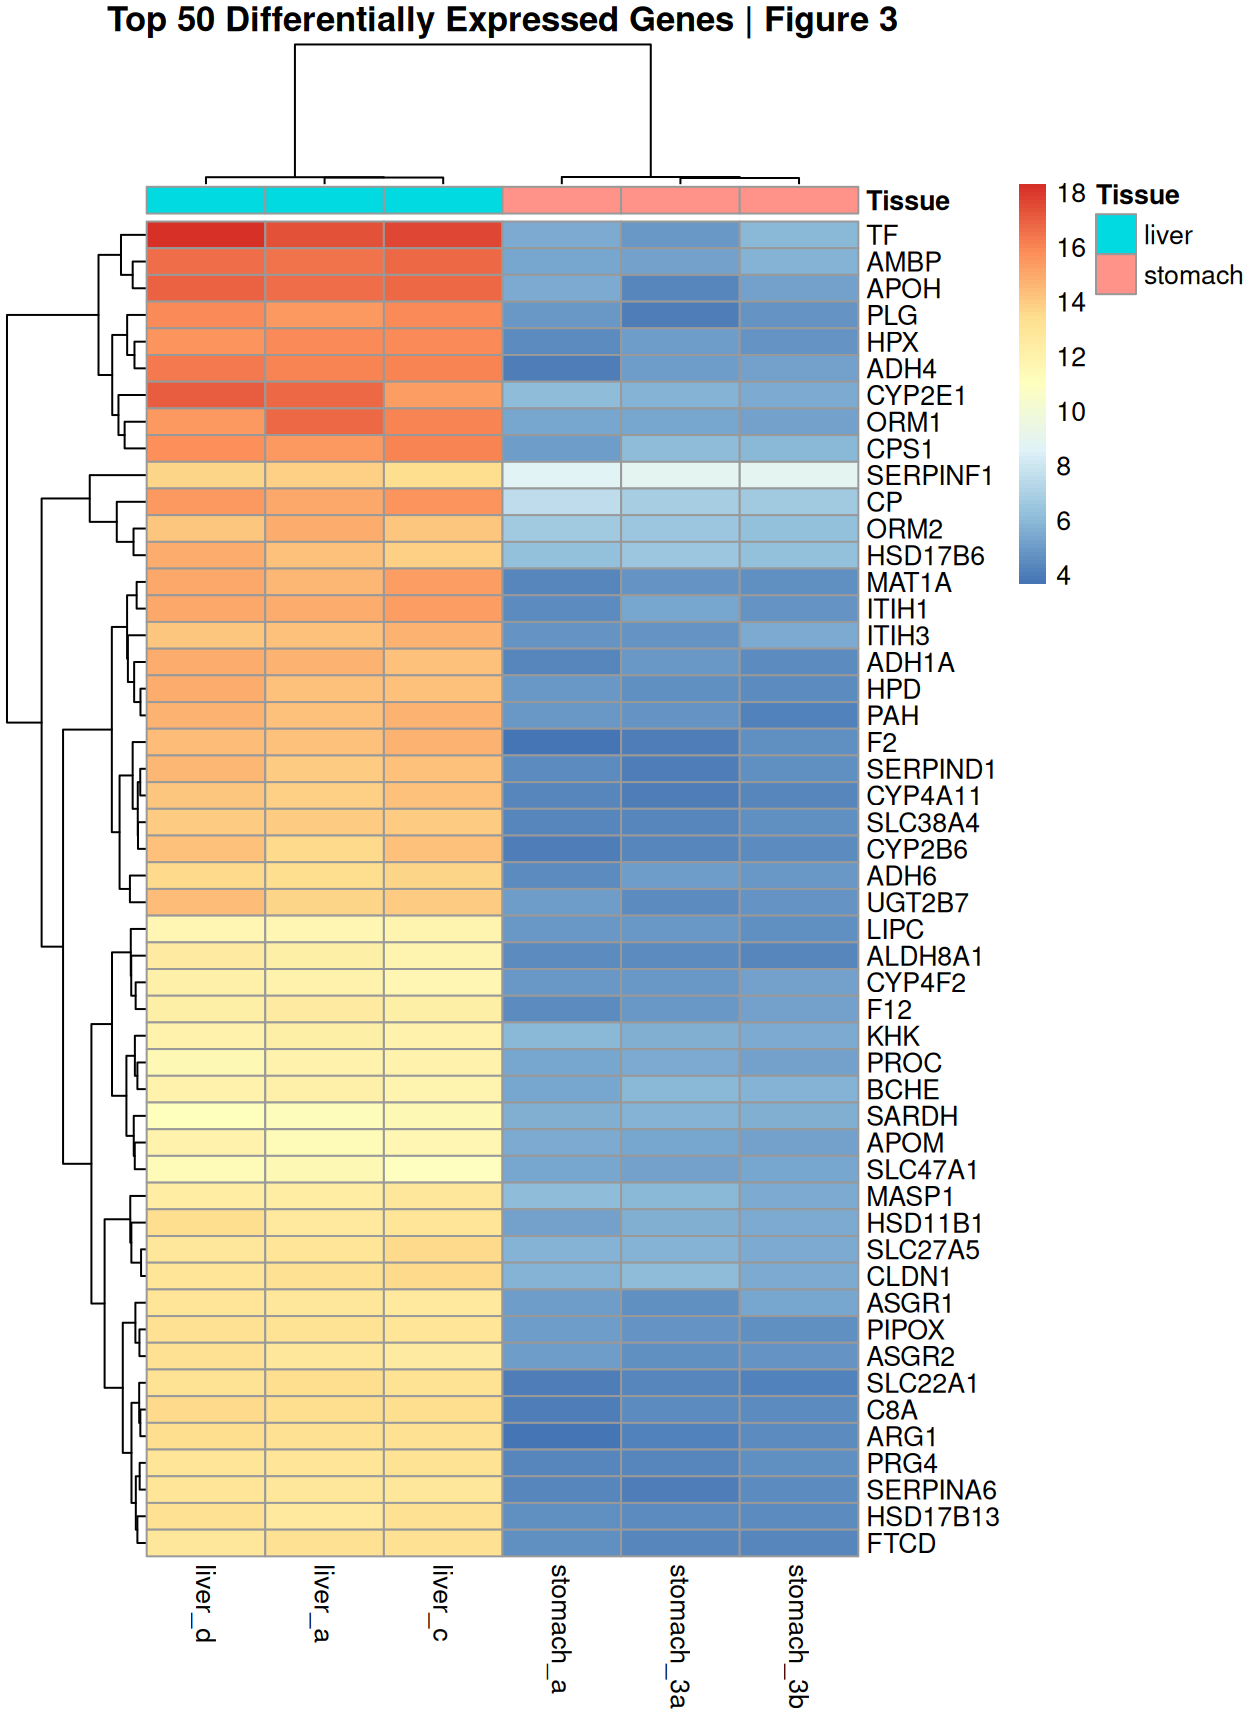
\includegraphics{InterimAnalysis_files/figure-latex/fig3_geneHeatmap-1.pdf}
Pretty much all of the top genes were more directly associated with
liver specific functions. Some of the liver functions highlighted by
these genes were detoxification enzymes, lipid metabolism, and metabolic
enzymes.

One gene that stands out as the most significant for stomach tissue is
`SERPINF1'. The gene encodes a protein PEDF known for being an potent
inhibitor of angiogenesis a process of forming new blood vessels from
existing blood vessels. Another role is as an anti-inflammatory and
anti-oxidative stress agent. This is especially important in the liver
but also in the stomach as both organs are exposed to damaging
substances (Gattu 2013).

The next step was to determine the top genes differencially expressed
for each tissue type. The goal here is to determine if there are any
gene similarly expressed genes based on the top genes for each tissue.
This will help shed more light on the top expressed genes from stomach
tissue samples because overall there was less differentially expressed
genes for this type.

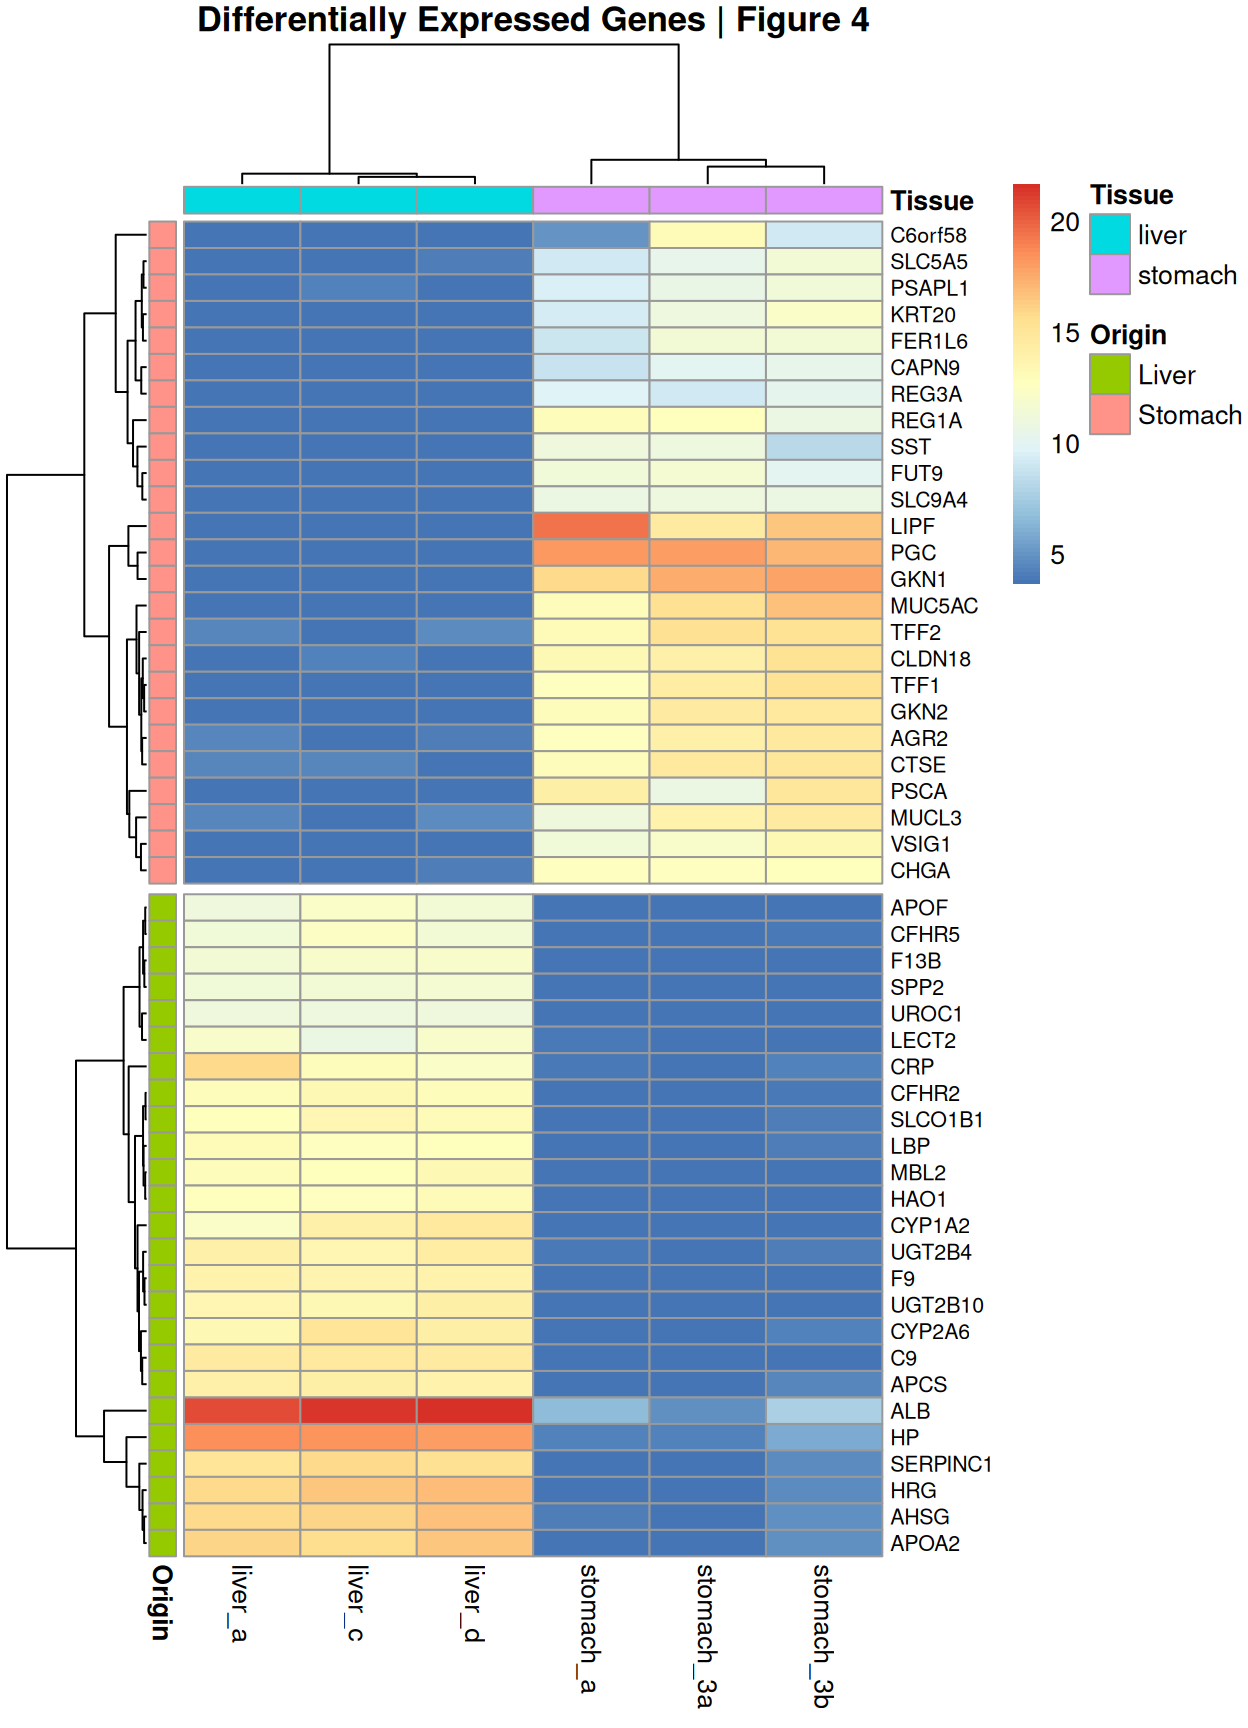
\includegraphics{InterimAnalysis_files/figure-latex/fig4_geneHeatmap2-1.pdf}
Moreover, this heatmap continues to confirm the hypothesis of the
distinct ``filtering'' function differences of the liver and stomach.
There are two distant clusters once again with no specific gene showing
expression in both tissue type.

\textbf{Liver-Specific Genes:} ALB: Albumin, the most abundant protein
in blood plasma, produced almost exclusively by the liver\\
SERPINC1: Antithrombin, a serine protease inhibitor that regulates blood
coagulation HP, HRG, AHSG, APOA2

\textbf{Stomach-Specific Genes:} MUC5AC and MUC3, GKN1 and GKN2, CLDN18,
PSCA, VSIG1, TFF1 and TFF2: Trefoil factors involved in mucosal
protection and repair

Next, a more targeted approach was taken to use a pre-defined list of
important genes related to each tissue type. These genes were taken from
a various of research publications based on their importance in the
various functions of their respective organ. These pre-defined genes can
be found LISTED HERE.

Using these genes one last heatmap was created to see if there is any
expression between even more specific genes.

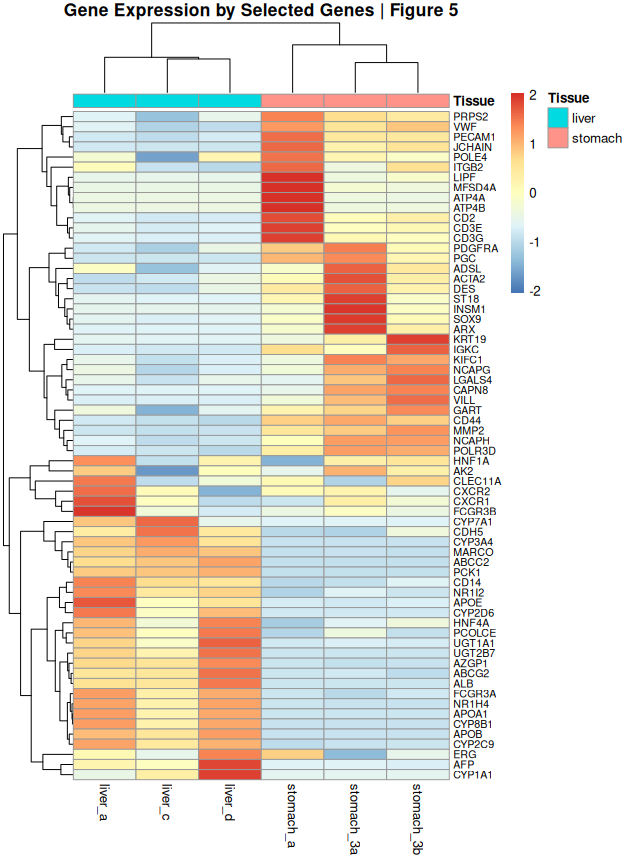
\includegraphics{InterimAnalysis_files/figure-latex/fig5_geneHeatmap3-1.pdf}
The top right cluster represents that of stomach related genes. The
bottom left cluster represents that of genes are the liver related. Once
again we can see two distinct clusters. There is very few overlap in
expression between the two tissue types.

\subsection{Enrichment Analysis}\label{enrichment-analysis-1}

--NOT DONE--

\newpage

\section{-- Outline --}\label{outline}

\section{Abstract}\label{abstract}

\section{Introduction}\label{introduction-1}

\subsection{Sample Selection}\label{sample-selection}

\subsection{Hypothesis}\label{hypothesis-1}

\section{Methods}\label{methods-1}

\subsection{Qualitiy Analysis}\label{qualitiy-analysis}

\subsection{Trimming}\label{trimming-1}

\subsection{Mapping}\label{mapping-1}

\subsection{Counting}\label{counting}

\subsection{Statistical Analysis}\label{statistical-analysis}

\subsubsection{Heatmap}\label{heatmap}

\subsubsection{PCA}\label{pca}

\subsubsection{Gene Heatmap}\label{gene-heatmap}

\subsubsection{Pathway / GO enrichment}\label{pathway-go-enrichment}

\section{Results}\label{results-1}

\section{Discussion}\label{discussion}

\section{Conclusion}\label{conclusion}

\section{References}\label{references}

Gattu, A. K., Swenson, E. S., Iwakiri, Y., Samuel, V. T., Troiano, N.,
Berry, R., Church, C. D., Rodeheffer, M. S., Carpenter, T. O., \& Chung,
C. (2013). Determination of mesenchymal stem cell fate by pigment
epithelium-derived factor (PEDF) results in increased adiposity and
reduced bone mineral content. FASEB journal : official publication of
the Federation of American Societies for Experimental Biology, 27(11),
4384--4394. \url{https://doi.org/10.1096/fj.13-232900}

Mills, J. C., \& Shivdasani, R. A. (2011). Gastric epithelial stem
cells. Gastroenterology, 140(2), 412--424.
\url{https://doi.org/10.1053/j.gastro.2010.12.001}

Rui L. (2014). Energy metabolism in the liver. Comprehensive Physiology,
4(1), 177--197. \url{https://doi.org/10.1002/cphy.c130024}

\end{document}
